\newpage


\section{Existujúce riešenia}

Existuje veľké množstvo riešení problému s dynamickým odporúčaním. Všetky pracujú s nejakou množinou vlastností, tém alebo kľúčových slov, ku ktorým sa snažia vypočítať pravdepodobnosť, že práve daná téma, kľúčové slovo alebo vlastnosť je pre používateľa najzaujímavejšia a následne mu odporučiť vyhľadávané subjekty, z danou vlastnosťou.

Postup riešenia sa dá rozdeliť na niekoľko podproblémov, ktoré sa dajú riešiť osobitne:

\begin{itemize}
\item{získavanie vlastnosti dokumentov,}
\item{získavanie používateľskej spätnej väzby,}
\item{ukladanie používateľského profilu,}
\item{porovnávanie používateľových preferencií s dokumentami,}
\item{starnutie preferencií,}
\item{triedenie preferencií na krátkodobé a dlhodobé,}
\end{itemize}

\subsection{Kategorizácia dokumentov}

Aby sme mohli odporučiť dokument, musíme získať nejaké jeho vlastnosti, ktoré budeme vedieť priradiť k používateľskému profilu. 

\paragraph{Kategorizovanie na základe typu dokumentu}

Prvou skupinou vlastností určujúcich dokument je jeho typ. Dokumenty môžu byť piatich typov, pričom sú možné aj rôzne kombinácie typov, teda môže nastať, že mám text s akordmi pričom sólo daného hudobného diela je zapísané pomocou tabov. Takže pre každý dokument \(d_j\) z množiny dokumentov \(D = (d_0, d_1, \cdots, d_n)\) budem mať určené štyri premenné \(d_j = (a_j, x_j, p_j, t_j, n_j)\), ktoré budú nadobúdať buď hodnotu \(1\) alebo \(0\) na základe toho, či dokument patrí do danej kategórie alebo nie. Jednotlivé premenné reprezentujú nasledovné druhy obsahu:

\begin{itemize}
\item{\(a_j\) určuje či dokument \(j\) obsahuje akordy,}
\item{\(x_j\) určuje či dokument \(j\) obsahuje text,}
\item{\(p_j\) určuje či dokument \(j\) obsahuje preklad textu,}
\item{\(t_j\) určuje či dokument \(j\) obsahuje taby,}
\item{\(n_j\) určuje či dokument \(j\) obsahuje noty,}
\end{itemize}

\paragraph{Kategorizovanie na základe hudobnej štruktúry}

Hudobné dokumenty sa dajú ďalej deliť z hľadiska hudobnej štruktúry. Pre dokument \(d_j\) vieme určiť niekoľko časti štruktúry, Jeden hudobný dokument nemusí obsahovať všetky súčasti hudobného diela. Tak isto jedno hudobné dielo nemusí používať všetky štandardné súčasti. V zásade rozoznávame a určujem tieto štandardné časti hudobných diel \cite{1}:

\begin{itemize}
\item{predohra,}
\item{medzihra,}
\item{refrén,}
\item{ukončenie (angl. Outro),}
\item{sólo alebo inštrumentálna časť}\ignore{Nájdi článok,}
\end{itemize}

No toto nie je najmenšie možné delenie, z hľadiska kompozície môžeme ešte hudobné dielo rozdeliť na jednotlive nástroje, ktoré vykonávajú dané prevedenie hudobného diela. Tak isto sa dané časti môžu rozlišovať variáciami motívu\cite{12},

\paragraph{Kategorizovanie na základe prevedenia}

Ďalej môžeme hudobné diela deliť na základe konkrétneho prevedenia. Niektoré hudobné diela môžu mať aj niekoľko prevedení. Prevedenia sa dajú charakterizovať na základe miesta, použitých nástrojov alebo hudobníkov, ktorí dané prevedenie zahrali.

\paragraph{Kategorizovanie na základe žánru}

Žáner je asi jeden z najdôležitejších spôsobov kategorizovania hudobných diel. Hlavnými ukazovateľmi žánru hudobného diela sú akustické vlastnosti zvuku a téma textu. Momentálne existuje veľké množstvo hudobných štýlov a spôsobov zaradenia, avšak chýba určitá štandardizácia. Následkom toho či už automatické určovanie alebo určovanie bežným človekom dosahuje asi presnosť 70\% \cite{5}.Tak isto z hľadiska kompozície, každá časť hudobného diela môže obsahovať iný hudobný žáner\cite{3}.

\subsection{Získavanie používateľskej spätnej väzby}

Aby sme mohli presne určiť či daný hudobný dokument vyhovuje používateľovi, je potrebné nejakým spôsobom získať jeho spätnú väzbu. V zásade existujú dva spôsoby získavania spätnej väzby:

\begin{itemize}
\item{explicitná (používateľ vedome poskytne spätnú väzbu napr. hodnotenie dokumentu),}
\item{implicitná (používateľ o tejto spätnej väzbe nevie, používajú sa agenti ktorí ho monitorujú napr. počítanie času stráveného na stránke),}
\end{itemize}

\paragraph{Identifikácia používateľa}

Prvým krokom pri získavaní spätnej väzby je identifikácia používateľa, najpoužívanejší spôsob identifikácie používateľa je pomocou prihlásenia, kedy používateľ pred použitím systému identifikuje sám seba podľa mena a hesla. Tento spôsob sa radi medzi spôsoby ktoré vyžadujú zásah používateľa. 

Ďalšou alternatívou v tomto smere je softvérový agent, ktorého si používateľ nainštaluje u seba na počítači. Nevýhodou oproti predchádzajúcemu prístupu je že používateľ musí agenta nainštalovať na každom zariadení ktoré používa.

Alternatívy ktoré nevyžadujú používateľov zásah sú pomocou súborov cookie \ignore{Nájdi ako preložiť} a pomocou relácií. Obidve tieto alternatívy trpia tím že ak sa používateľ pristupuje z iného zariadenia nebudú ho vedieť identifikovať\cite{4}.

\subsection{Profil používateľa}

Rozlišujeme niekoľko druhov používateľských profilov, základe delenie je minimálny (angl. core) a rozšírený (angl. extended) profil. Minimálny používateľsky profil obsahuje čisto informácie o používateľových preferenciách, zatiaľ čo rozšírený používateľský profil obsahuje aj demografické informácie (vek, rodná krajina, vzdelanie, schopnosti atď,)\cite{4}

\paragraph{Model profilu používateľa}

Je viacero spôsobov ako uložiť profil používateľa, každý má svoje špecifiká a umožňuje iným spôsobom vykonávať odhadovanie používateľových záujmov.

\paragraph{Profil kľúčových slov(angl. keywords profiles)}

Profil kľúčových slov je matica o dimenziách používatelia x kľúčové slová. Na základe toho aké jednotlivé súradnice matice môžu dosahovať hodnoty 0 ak dané kľúčové slovo patrí do používateľovho profilu a 0 ak nie. Na obrázku 1. môžeme vidieť príklad v ktorom máme používateľa Používateľ 0 ktorý nemá žiadne kľúčové slová, následne Používateľa 1 ktorý používa kľúčové slová 1 a 2 a Používateľa 2 ktorý používa kľúčové slovo 1.

\begin{figure}
	\begin{center}
		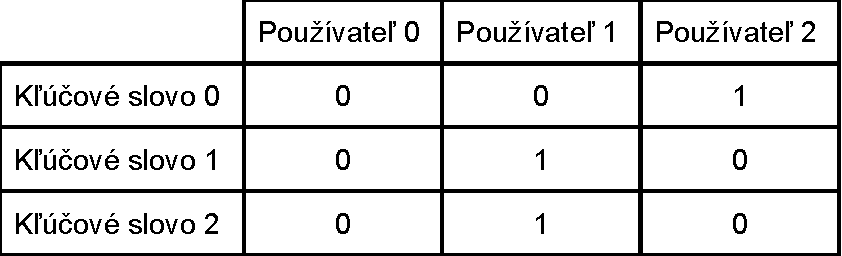
\includegraphics[scale=0.55]{keywordprfile}
		\caption{Ukážka profilu kľúčových slov.}
			\label{Profil klúčovích slov}
	\end{center}
\end{figure}

\paragraph{Profil sémantickej siete (angl. Semantic network profile)}

Tento tip profilu sa používa najmä v systémoch používajúcich rozširovanie používateľských vyhľadávacích reťazcov. Základom tohoto profilu je sémantická sieť ktorej príklad môžeme vidieť na obrázku 2.

\begin{figure}
	\begin{center}
		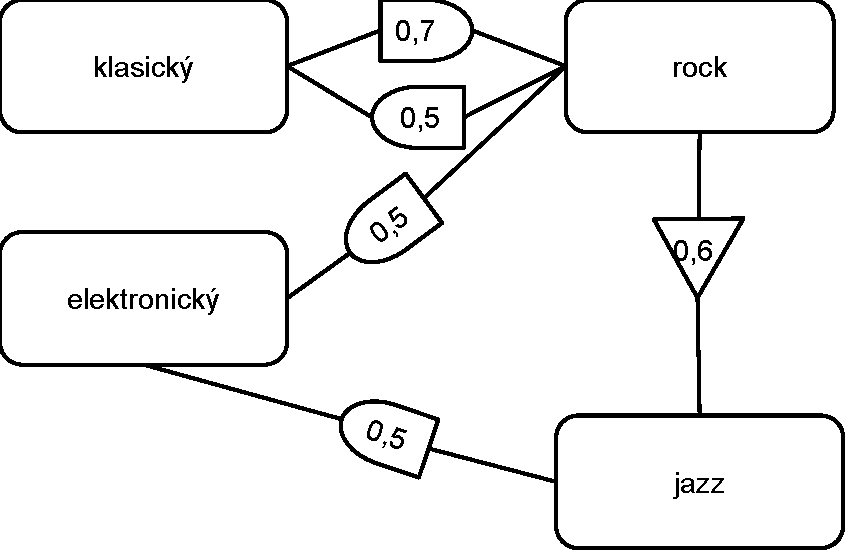
\includegraphics[scale=0.55]{semanticnetwork}
		\caption{Ukážka sémantickej siete}
	\end{center}
\end{figure}

Sémantická sieť je orientovaný graf v ktorom vrcholmi sú preferencie alebo vlastnosti dokumentov, zatiaľ čo hrany sú ich vzťahy. Vzťahy môžu byť niekoľkých typov:

\begin{itemize}
\item{konjunkcia,}
\item{disjunkcia,}
\item{substitúcia,}
\item{negácia,}
\end{itemize}

\subsection{Starnutie profilu}

Keďže používateľové zaujmi sú dynamické a menia sa v čase, môžeme implementovať niekoľko modelov starnutia preferencií.

\paragraph{Polia-urn model\ignore{prelož}}

Mám množinu záujmov \(D = (d_0, d_1, \cdots d_n)\), pre každý záujem \(d_j\) ukladám počet vybratí daného záujmu \(s_j\). Pravdepodobnosť znovu vybratia záujmu dostanem pomocou:

\[\frac{s_j}{\sum\limits_{i=1}^n s_i}\]

Kde n je rovné počtu záujmov. Tento model nezávisí od poradia v akom boli prejavené zaujmi.

Pravdepodobnosť že dosiahnem určitú kombináciu \(S = (s_0, s_1, \cdots ,s_n)\) je vyjadrená pomocou:

\[\frac{1}{\sum\limits_{i=1}^n s_i}\]

\cite{6}

\paragraph{Polčas rozpadu}

Jednou z možností ako zabezpečiť starnutie používateľského profilu je využiť funkciu exponenciálneho polčasu rozpadu. Táto funkcia sa hlavne využíva pri datovaní veku uhlíka, avšak dá sa použiť aj ako funkcia starnutia používateľových preferencií. Základom tohoto prístupu je následujúci vzorec:

\[N(t) = N_0e^{-k/t}\]

Aby sme mohli tento algoritmus použiť, musíme si určiť polčas rozpadu preferencie. Následne si na základe polčasu rozpadu vypočítam parameter \(k\), Ten sa dá po odvodení určiť z následujúceho vzorca.

\[k = \frac{\ln{\frac{1}{2}}}{t_r}\]\cite{7}

Kde \(t_r\) je polčas rozpadu. Tento model umožňuje vytvorenie viacerých rýchlosti starnutia pre krátkodobe a dlhodobé záujmy\cite{8}.


\subsection{Geometrické porovnávanie vlastnosti dokumentov z preferenciami}

Pri tomto spôsobe sa relevancia dokumentu \(d_i\) pre používateľa \(u_j\) bude určovať premietnutím dokumentu do priestoru ako vektor \(d_j=(p_0, p_1\cdots p_n)\) kde \(p_0, \cdots p_n\) sú vlastnosti dokumentu, následne sa do toho istého priestoru premietne aj používateľ, pričom dimenzie budú preferencie používateľa \(u_i=(p_0, p_1 \cdots p_n)\). Podobnosť týchto vektorov sa následne vyhodnotí pomocou nasledujúceho vzorca:

\[cos \theta = \frac{d_j * q}{||d_j||*||q||}\]

Pričom \(||d_j||\) a \(||q||\) sú normalizované vektory\cite{9}.


\subsection{Kolaboratívne filtrovanie}

Kolaboratívne filtrovanie je postup pri ktorom odporúčam používateľovi na základe podobnosti z iným používateľom. Kolaboratívne filtrovanie sa delí na založené na obsahu a kolaboratívne filtrovanie  \cite{10}.

Odporúčanie založené na obsahu vychádza z dostupných informácií o diele, teda z vlastnosti diela zatiaľ čo kolaboratívne filtrovanie záleží čisto od explicitnej spätnej väzby používateľa pomocou hodnotenia.

Podľa \cite{10} dosahuje kolaboratívne filtrovanie väčšiu dynamiku. Avšak hrozí problém studeného štartu, teda že novo pridaná položka nebude mať žiadne hodnotenie a preto klesne hneď na spodok odporúčaní. Kolaboratívne filtrovanie môžeme ďalej rozdeliť:

\begin{itemize}
\item{kolaboratívne filtrovanie založené na pamäti}
\item{kolaboratívne filtrovanie založené na modeli}
\item{hybridné kolaboratívne filtrovanie \cite{11}}
\end{itemize}

\paragraph{Kolaboratívne filtrovanie založené na pamäti}

Podobnosť medzi používateľmi sa zisťuje na základe hodnotenia dokumentov. Je použitá heuristicka metóda ktorá zisťuje chýbajúce hodnotenia porovnávaním používateľov a následne doplnenie od najpodobnejšieho používateľa.

\paragraph{Kolaboratívne filtrovanie založené na modeli}

Pracuje z modelom ktorí vytvára hodnotenie a súčasne sa učí na existujúcich dátach.

\paragraph{Hybridné kolaboratívne filtrovanie}

Na obídenie nedostatkov algoritmov kolaboratívneho filtrovania, niektoré aplikácie kombinujú tieto dve metódy.

\section{Logistická funkcia}

Logisticka funkcia sa často používa ako pravdepodobnostná funkcia. Funkcia má nasledujúci tvar: 

\[f(t; a,m,n,\tau) = a*\frac{1 + me^{-t/\tau}}{1 + ne^{-t/\tau}}\]

Vo väčšine prípadov sa používa špecialny prípad tejto funkcie meno signusoida.
Signusoida ma $a = 1$, $m = 0$, $n = 0$ a $\tau = 1$ čiže:

\[f(t) = \frac{1}{1 + e^{-t}}\]

Graf tejto funkcie má tvar písmena S


%\subsection{Evolúcia používateľských profilov}
%
%Evolúcia používateľských profilov je modelovaná pomocou dynamických Bayesianskych sieti (angl. Bayesian networks). Tieto siete reprezentujú dočasné závislosti medzi interakciami v rôznych časoch, to znamená že ak máme sekvenciu používateľových interakcií modelovanú modelmi Bayesianskych sieti pre rôzne časove úseky \( \in [0..T-1], \text{ teda } I_0, I_1, I_2, \ldots I_{T-1} \), použili sme dočasne odkazy na prepojenie uzlov v Bayesianskej sieti cez rôzne časove úseky.
%
%Súčasť modelu sa skladá zo sekvencií náhodných premenných S, I a Du pre T po sebe idúcich časových úsekov \[t \in [0..T-1].\]. \ignore{FIXME čo znamená táto veta ?}S S, I a Du označujú poradie vyhľadávania v relácií, interakcie používateľa a zostávajúci čas v čase t. Každá interakcie používateľa zo systémom je modelovaná ako orientovaný acyklický graf zložený z dvoch množín, množina vrcholov V a množina hrán E. Každá hrana reprezentuje vzťah medzi dvoma vrcholmi.
%
%\paragraph{Popis pravdepodobnosti}
%
%V tejto sekcií popíšeme pravdepodobnosti ktoré sú súčasťou modelu.
%
%\paragraph{Vyhľadávacia relácia}
%
%Nech \(S = {1, \cdots m,\cdots, M}\) je množina M vyhľadávacích relácií, kde náhodná premenná \(S_t\) má hodnotu. Pravdepodobnosť relácie je definovaná pre každé \(m \in S\) pomocou
%
%\[P(S_t = m) = v_{t,m}q\]
%
%Kde \(v_{t,m}\) je pravdepodobnosť že relácia m je v čase t. Rozdelenie pravdepodobnosti \(v_t\) je vektorový súčet M elementov (M=počet relácií).
%
%\paragraph{Pravdepodobnosť počiatočnej interakcie}
%
%Uvažujeme N používateľových interakcií, kde náhodná premenná \(I_t\) berie hodnotu v \(I = {1, 2\cdots N}\).
%Každá používateľova interakcie zo systémom v čase t, preskupí dotaz \(q_t\) a odvodený používateľov záujem zapísaný \(c_{k,t}\) a je reprezentovaný trojicou < Q, C, F > kde \(Q=q_t\) reprezentuje dotaz odoslaný počas interakcie. \(C=c_t\) reprezentuje používateľov profil definovaný jeho záujmom and F je funkcia relevancie ktorá určí relevanciu dokumentu \(d_j\) z prihliadnutím na používateľov záujem \(c_k\) a dotaz \(q\), popísaný ako:
%
%\[F(g,d_j,c_k)=P(d_j/q)\times P(c_k/q)\times P(q)\]
%
%Výsledná pravdepodobnosť pre každý dotaz \(q\) v inštancií každého dokumentu \(d_j\) a záujem \(c_k\) sú reprezentované v matici \(X_{n,m}\) o dimenziách (počet dokumentov x počet používateľových záujmov) 
%
%Avšak pravdepodobnosť počiatočnej používateľovej interakcie \(P(I_0=n)\) preskupujúca dotaz \(q_0\) odoslaný v čase \(t=0\) a používateľov záujem \(c_{k,0}\) odvodený v čase \(t=0\) podľa vyhľadávacej relácie je definovaný:
%
%\[P(I_0=n|S_0=m)=P(q_0, c_{k,0}|S_0=s)=A_{0,m,n}\]
%
%Kde \(A_{0,m,n}\) udáva pravdepodobnosť začatia používateľovej interakcie \((I_0=n)\) udávajúca počiatočnú reláciu \((S_0=m)\). Rozdelenie pravdepodobnosti \(A_0\) je matica M(počet relácií) riadkov a N(počet interakcií) stĺpce.
%
%\paragraph{Pravdepodobnosť počiatočného času pobytu}
%
%Pravdepodobnosť času pobytu rozloženie času stráveného v každej možnej (relácií, používateľovej interakcie) konfigurácií. Nech \(Du = {1\cdots d, \cdots , D}\) kde náhodná premenná \(Du_t\) nadobúda hodnotu, s \(D\) označujúcim maximálny počet časových jednotiek, ktoré môže akákoľvek konfigurácia relácie a interakcie trvať. Pre počiatočnú interakciu \(I_0=n\) a reláciu \(S_0 = m\), pravdepodobnosť počiatočného času pobytu je daná pomocou:
%
%\[P(Du_0=d|I_0=n, S_0=m)=L_{0,n,m,d}\]
%
%Kde \(L_{0,n,m,d}\) je pravdepodobnosť strávenia \(d\) časových jednotiek v počiatočnej interakcií a konfigurácií relácie. Toto je reprezentované ako matica NM(počet interakcií x počet relácií) riadky a D stĺpce (počet časových jednotiek).
%
%\subsection{TVUM}
%
%Mám \(n_{ik}\) reprezentujúce počet akcií opsujúcich zaujem k používateľa i. Používateľ buď zopakuje akciu z pravdepodobnosťou závislou na \(n_{ik}\) alebo začne pracovať z úplne novím záujmom \(\lambda\).
%Nový záujem je rozhodnutý na základe globálnych frekvencií záujmov.
%
%Nech \(m_{k}\) reprezentuje frekvenciu z akou je záujem \(k\) populárny o používateľov.
%
%Delenie používateľovích do ``epoch''.
%
%Používateľové akcie v každej epoche sú modelované pomocov epoch-specific, fixný počet stĺpcov hierarchycký polia-urn model.
%
%Používam polia-urn model, čo je verzia the chinese restaurant process zo sady dirichlet processes


%\subsection{Poznámky}

%Jeden používateľ sa môže podobať druhému používateľovy z pred pár rokov.


%\paragraph{Kontext}
%
%Používatelia môžu mať v rôznych kontextoch rôzne ciele, čo by sa malo dať zohladniť v rámci vyhľadávania. Problém je, ako zistiť v akom kontexte sa nachádzam.


%\paragraph{Nadpis ešte nižšej hierarchie}\label{nadpis75}
%orbi sagittis luctus \emph{risus}\footnote{\emph{slov.} smiech} molestie mattis. Cras turpis mauris, lacinia a eleifend in, semper a augue. Aenean ultrices rhoncus metus ut auctor. Pellentesque fermentum justo eget erat commodo vel mollis augue semper. Nunc tempor augue nulla, pellentesque posuere orci\footnote{viac v kap. \ref{podsekcia2}}.

%Cum sociis natoque penatibus et magnis dis \emph{parturient montes}, nascetur ridiculus mus. Integer turpis lacus, convallis porta aliquam eu, luctus in orci. Duis tincidunt condimentum augue in laoreet. Vivamus tempus iaculis ligula, dictum dignissim nibh elementum at. Donec quis risus quis sem blandit auctor. Integer eu tellus nisi, et fringilla magna. Praesent vulputate placerat pretium. Etiam vitae ornare est.\\


%\begin{lstlisting}[float=h,caption={Príklad listingu priamo v latex-u}, label={listing2},
%	keywordstyle=\color{blue}\bfseries, ndkeywordstyle=\color{black}\bfseries, commentstyle=\color{red}\ttfamily,
%	stringstyle=\color{green}\ttfamily, identifierstyle=\color{gray},backgroundcolor=\color{white},frame=single, frameround=ffff,captionpos=b,basicstyle=\scriptsize]
%	Aenean consequat
%	sapien a posuere
%	tincidunt massa
%	purus egestas nisl
%	sed sollicitudin
%	neque mi vel augue.
%\end{lstlisting}
%
%\begin{my_description}
%	\item {\textbf{položka 1} - Tuto nasleduje popis položky 1.}
%	\item {\textbf{položka 2} - Tuto nasleduje popis položky 2.}
%	\item {\textbf{položka 3} - Tuto nasleduje popis položky 3.}
%\end{my_description}
%
%\subsubsection{Ďalšia podsekcia}
%Cum sociis natoque penatibus et magnis dis parturient montes, nascetur ridiculus mus. Integer turpis lacus, convallis porta aliquam eu, luctus in orci. Duis tincidunt condimentum augue in laoreet. Vivamus tempus iaculis ligula, dictum dignissim nibh elementum at. Donec quis risus quis sem blandit auctor. Integer eu tellus nisi, et fringilla magna. Praesent vulputate placerat pretium. Etiam vitae ornare est~\cite{2}.\\
%
%\begin{figure}[H]\begin{center}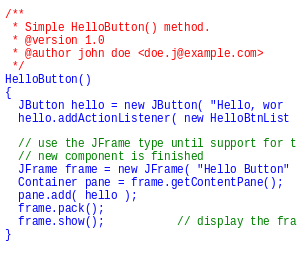
\includegraphics[scale=0.6]{figure1}
%\caption{Popis obrázku.}\label{figure1}\end{center}\end{figure}

%Pellentesque id sem sed nulla vehicula pellentesque. Vestibulum tincidunt faucibus tortor, et feugiat libero sagittis eget. Maecenas ultrices justo venenatis lectus malesuada gravida. Quisque commodo auctor sem, ut congue dolor ullamcorper sit amet. Sed eu dolor purus. Aliquam blandit, magna sed gravida ultrices, nibh mi porttitor erat, sed scelerisque enim magna nec risus. Mauris vestibulum arcu vel enim rhoncus eleifend. Sed nec interdum sapien. Pellentesque tincidunt condimentum consectetur. Maecenas posuere nunc in lacus consectetur sed posuere felis tristique. Vivamus diam lorem, commodo eget aliquet sed, volutpat sit amet nisi. Morbi posuere leo sit amet odio dignissim hendrerit. Praesent eget urna odio, non hendrerit neque. Suspendisse eget massa metus, in vestibulum est. Donec ac elit vitae ante auctor laoreet. Donec purus lorem, bibendum vel euismod ac, semper quis lacus~\cite{3}.

%\begin{figure}[H]\begin{center}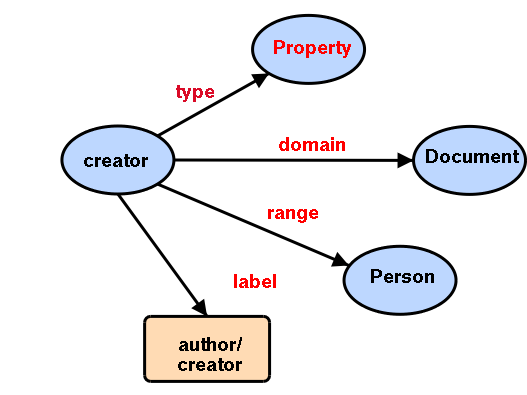
\includegraphics[scale=0.6]{figure2}
%\caption{Popis obrázku; prevzaté z~\cite{3}.}\label{pic1}\end{center}
%\end{figure}

